\documentclass[spanish]{beamer}
\usepackage[spanish]{babel} %esto es para que las ondas estn en espaol

% Vary the color applet  (try out your own if you like)
%\colorlet{structure}{red!65!black}

%\beamertemplateshadingbackground{yellow!100}{white}

\usepackage[utf8x]{inputenc}
\usetheme{Madrid} 

\usepackage{beamerthemesplit}
\usepackage{graphics}
\usepackage{graphicx}
\usepackage{hyperref}
\usepackage{amsfonts}
\usepackage{listings}
\usepackage{color}
\definecolor{dkgreen}{rgb}{0,0.6,0}
\definecolor{gray}{rgb}{0.5,0.5,0.5}
\definecolor{mauve}{rgb}{0.58,0,0.82}

\lstdefinelanguage{Java}{
  morekeywords={class,struct,true,false,void,%
    if,else,while,return,int,char,boolean},
  otherkeywords={{,},;,+,-,/,*,<=,>,<,<=,>=,!=,==,\%,@},
  sensitive=true,
  morecomment=[l]{//},
  morecomment=[n]{/*}{*/},
  morestring=[b]",
  morestring=[b]',
  morestring=[b]"""
}

\lstset{frame=tb,
  language=Java,
  aboveskip=3mm,
  belowskip=3mm,
  showstringspaces=false,
  columns=flexible,
  basicstyle={\small\ttfamily},
  numbers=none,
  numberstyle=\tiny\color{gray},
  keywordstyle=\color{blue},
  commentstyle=\color{dkgreen},
  stringstyle=\color{mauve},
  frame=none,
  breaklines=true,
  breakatwhitespace=true
  tabsize=3
}

\lstset{language=Java}

\title[MapReduce]{MapReduce en Sistemas Distribuídos}
\author[Hector Hurtarte,Carlos L\'{o}pez Camey]{%
  Hector Hurtarte \and
  Carlos L\'{o}pez Camey}
\institute[Universidad del Valle de Guatemala]{
  CC3008 - Sistemas Operativos Avanzados \\
  Departamento de Ciencias de la Computaci\'{o}n \\
  Universidad del Valle de Guatemala}
\date[Investigaci\'{o}n 1]{Investigaci\'{o}n 2 - Sistemas distribuídos}

\subject{MapReduce}

\begin{document}
  \frame{
    \titlepage
  }

  \section{Introducción}
  \subsection{Resumen}
  \frame{
    \frametitle{Resumen}
    
    MapReduce es un modelo de programación ampliamente usado en sistemas distribuídos para procesamiento de datos a larga escala. 
    El modelo consiste en definir:
    \begin{itemize}
    \item Una función \textbf{map}
    \item Una función \textbf{reduce}
    \item Paralelizar las tareas y balancear la carga entre nodos mediante un programa principal para obtener el resultado esperado.
    \end{itemize}
  }
        
  \section{Principios de programación funcional y ventajas}
  \subsection{Funciones map y reduce}
  \frame{
    \frametitle{La función Map}
    \begin{itemize}
      \item Generalmente definida sobre listas, pero puede actuar sobre otras estructuras e.g. Arrays, Secuencias, Sets, Iterables.
      \item Toma una lista de $A$'s ($[A])$ donde $A$ es un tipo y una función $f: A \rightarrow B$ (donde $B$ es otro tipo, no necesariamente el mismo) para regresar una lista de $B$'s ($[B]$)
      \item Firma de la función: $(A \rightarrow B) \rightarrow [A] \rightarrow [B]$
      \item Ejemplos:
        \begin{enumerate}
          \item $\textbf{map}( \lambda \: x. x + 5, [1,2,3,4..10] ) \Rightarrow [6,7,8,9..15]$ donde la función es $f: \mathbb{Z} \rightarrow \mathbb{Z}, f(x) = x + 5$, la lista que se quiere mapear es de Enteros y la evaluación resulta en otra lista de Enteros
          \item $\textbf{map}( \lambda \: x. x \cdot 2.0, [5,10,15,20]) \Rightarrow [10.0, 20.0, 30.0, 40.0]$, donde la función es $f: \mathbb{Z} \rightarrow \mathbb{R}, f(x) = x \cdot 2.0 $ y la lista que se quiere mapear es de Enteros y la evaluación resulta en una lista de Reales
        \end{enumerate}      
    \end{itemize}
  }

  \frame{
    \frametitle{Ejemplo en python}
    \lstinputlisting[language=Python,label=map.py]{programas-ejemplo/map.py}
  }

  \frame{
    \frametitle{La función Reduce}
    \begin{itemize}
      \item También definida sobre secuencias.
      \item Toma una lista de $A$'s, una función $f: (B,A) \rightarrow B$ para regresar un $B$, es decir, trata de \textit{reducirla} a un sólo valor (de tipo $B$).
      \item Firma de la función: $((B,A) \rightarrow B) \rightarrow [A] \rightarrow B$
      \item Ejemplo:
        \begin{enumerate}
          \item $\textbf{reduce}( \lambda \: x,y. x + y , [1,2,3,4,5]) \Rightarrow 15$. en donde la función toma dos argumentos de tipo entero y los suma $f: (\mathbb{Z},\mathbb{Z}) \rightarrow \mathbb{Z}$ y opera sobre la una lista de 1 a 5. 
            \begin{itemize}
              \item La función trata de reducir por tuplas de números ($\in \mathbb{Z}$) y empieza por un lado, por lo que si empezamos por la izquierda, tenemos en la primera operación: $1 + (2 + 3 + 4 + 5) = 1 + (2 + 3 + 9) = 1 + (2 + 12 = 1 + (14) = 15$
            \end{itemize}
        \end{enumerate}
    \end{itemize}
  }
  
  \frame{
    \frametitle{Ejemplo en python}
    \lstinputlisting[language=Python]{programas-ejemplo/reduce.py}
  }
  
  \subsection{Ventajas en un sistema distribuído}
  \frame{
    \frametitle{Programación funcional en sistemas distribuídos}
    \begin{itemize}
      \item Operaciones son \textit{side-effects free} (no tienen efectos secundarios)      
      \item Las funciones mantienen un \textit{estado}, donde el resultado de ésta función depende únicamente de sus variables libres. Ejemplo: f(x) = x + 5
      \item Los valores son inmutables i.e. no pueden cambiar de valor.
      \item Por lo tanto, pensando en \textit{thread-safety}, podemos decir que la programación funcional \textbf{promueve la exclusión mutua} en sistemas distribuídos.
    \end{itemize}
  }

  \frame{
    \frametitle{Ejemplo típico de programa con \textit{side-effects}}
    \lstinputlisting[language=Java]{programas-ejemplo/side-effects-presentacion1.java}
  }

  \frame{
    \frametitle{Ejemplo típico de programa con \textit{side-effects}}
    \lstinputlisting[language=Java]{programas-ejemplo/side-effects-presentacion2.java}
  }

  \section{Implementación y soluciones a problemas en sistemas distribuídos}
  \subsection{Entorno}
  \frame{
    \frametitle{Entorno}
	Considerese un sistema como el siguiente:
    \begin{itemize}
    	\item Muchas computadoras con procesador dual x86, Linux y 2-4 GB de memoria.
    	\item Conexión de 100 Mbps a 1 Gbps.
    	\item \textit{Clusters} con cientos o miles de computadoras (propenso a fallas).
    	\item \textit{Filesystem} distribuído con replicación (GFS).
    	\item Usuarios que presentan \textit{jobs} a calendarizador.
    \end{itemize}
  }
    
  \subsection{Implementación en sistemas distribuídos: Ejecuci\'{o}n }
  \frame{
    \frametitle{Implementación en sistemas distribuídos: Ejecuci\'{o}n 1/2}
   		\begin{center} 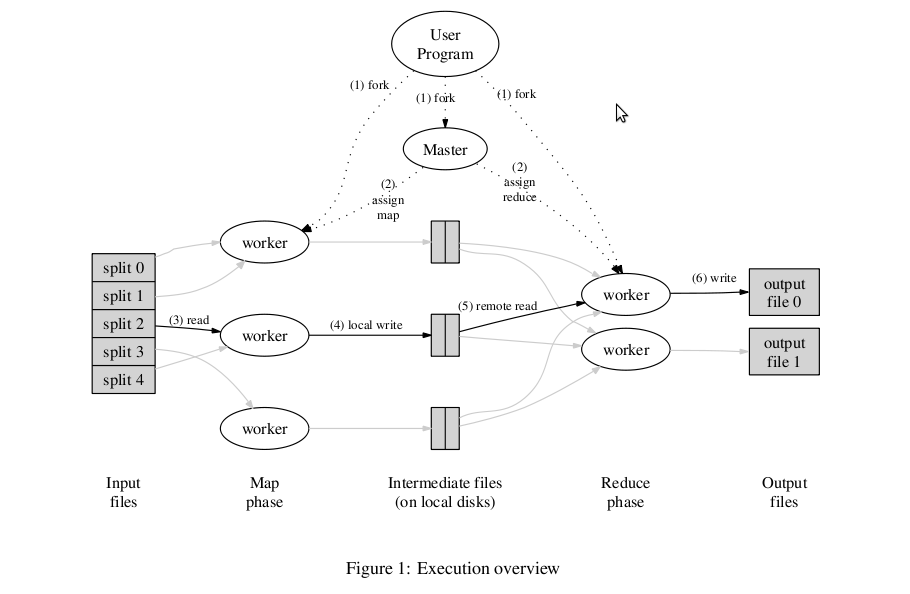
\includegraphics[width=10.5cm]{imagenes/ExecutionOverview.png} \end{center}
  } 
  
  \frame{
    \frametitle{Implementación en sistemas distribuídos: Ejecuci\'{o}n 2/2}
    	Invocaciones a \textit{Map} sobre {data} particionada en \textit{M} \textit{splits} (inmutables) que pueden ser procesados en paralelo. Invocaciones a \textit{Reduce} en \textit{R} equipos:
    	\begin{enumerate}
			\item \textit{Input} en \textit{M} particiones de 16 a 64 MB. Se hacen copias del programa. 
			\item \textit{Master} que asigna \textit{M} tareas \textit{Map} y \textit{R} tareas \textit{Reduce} a trabajadores \textit{idles}.
			\item Un trabajador obtiene pares (llave,valor) y alimenta función \textit{Map} que almacena pares intermedios en \textit{buffers} (se sobrepone a bugs!).
			\item \textit{Buffer} se traslada a discos locales, particionado en \textit{R} regiones y se notifica a \textit{master}.
			\item Un trabajador ordena y agrupa pares intermedios seg\'{u}n \textit{keys}.
			\item Se itera sobre la \textit{data} intermedia y se pasa un \textit{key} y su conjunto a la función \textit{Reduce}. Se producen salidas por cada partición de \textit{reduce}.
			\item Cuando todo ha finalizado se retorna al \textit{user program}.
		\end{enumerate}
  } 
	\frame{
		\frametitle{Execution2}
		   		\begin{center} 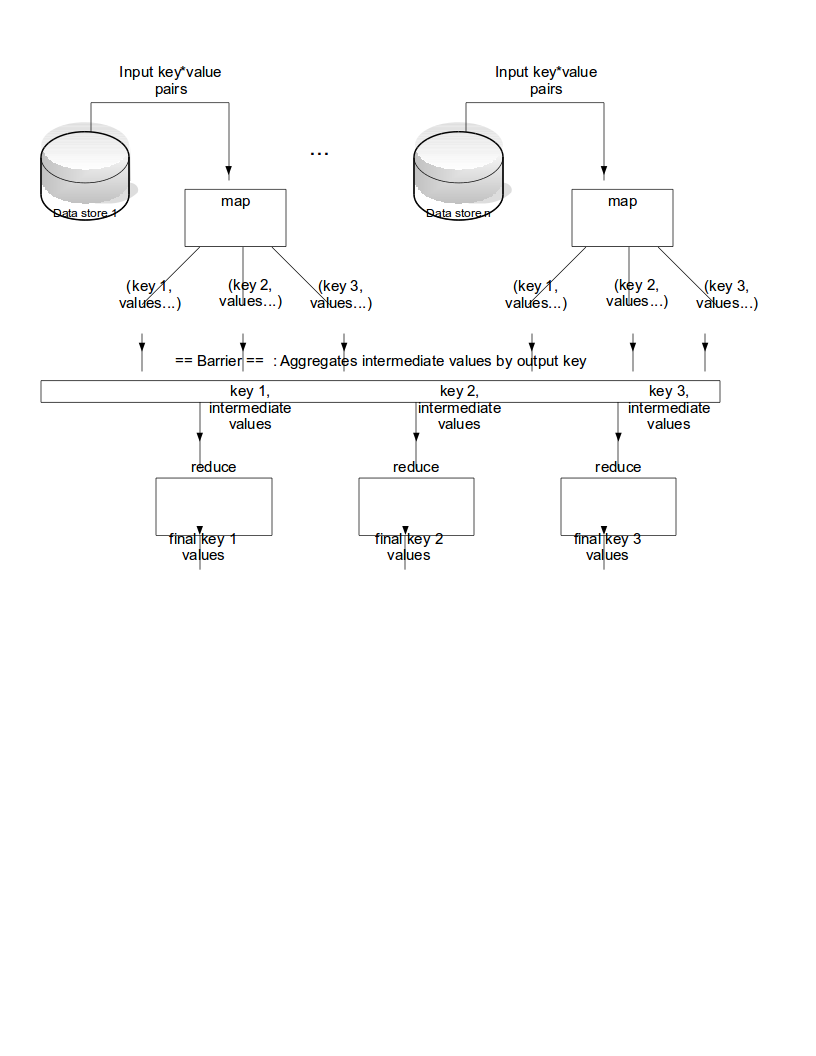
\includegraphics[width=7.5cm]{imagenes/ExecutionOverview2.png} \end{center}
	}  
  
  \subsection{Estructuras y parámetros}
  \frame{
    \frametitle {Estructuras y parámetros}
    	\begin{itemize}
		\item El proceso \textit{master} almacena:
    	\begin{itemize}
    		\item El estado para cada tarea (\textit{idle}, \textit{in-progress}, \textit{completed}).
    		\item Identidad de cada trabajador (para tareas no \textit{idle}.
    		\item Para cada tarea \textit{Map} completada, posici\'{o}n y tamaño de las \textit{R} regiones (archivos) producidas.
    	\end{itemize}
    	\item Cada proceso \textit{Map} devuelve a \textit{master} con el nombre de los \textit{R} archivos temporales generados.
    	\item Cada proceso \textit{Reduce} renombra sus archivos temporales.
    	\end{itemize}
  }
  
  \subsection{Balanceo, granularidad y complejidad}
  \frame{
    \frametitle{Balanceo, granulidad y complejidad}
    \begin{itemize}
    	\item \textit{Map} utiliza \textit{M} trozos y \textit{Reduce} \textit{R}. 
    	\item \textit{M} y \textit{R} $>>$ N. de trabajadores.
    	\item Obliga a que las tareas se repartan ámpliamente cuando uno falla (balanceo de carga).
    	\item \textit{O(M+R)} decisiones de calendarizaci\'{o}n, \textit{O(M $\cdot$ R)} estados en memoria.
    	\item \textit{R} tiende a limitarse, \textit{output} de cada \textit{reduce} termina en archivo separado.
    	\item Tendencia a escoger \textit{M} para que cada tarea utilize 16 a 64 MB y \textit{R} múltiplo de N. de trabajadores (aprox.). 
    \end{itemize}
  }

  \subsection{Tolerancia a fallas}
  \frame{
    \frametitle{Tolerancia a fallas}
    Las consideraciones del entorno obligan a una librería tolerante a fallas:
    \begin{itemize}
    	\item \textbf{Trabajador}. Si \textit{!Ping}: \textit{failed}, tareas (\textit{map} o \textit{reduce incompletas)} se marcan como \textit{idle} (recalendarización).
    	\item \textbf{\textit{Master}}. \textit{Checkpoints} de estructuras que facilitan nuevas copias. Solo un \textit{master}, menos posibilidad de fallas. Implementaci\'{o}n actual falla si falla \textit{master}.
    	\item \textbf{Consideraciones}: \textit{Commits} atómicos de tareas \textit{Map} y \textit{Reduce} (archivos temporales de salida) por parte del GFS.
	\end{itemize}
  }

	\subsection{Backup}
  \frame{
    \frametitle{Combatiendo stragglers: tareas de backup}
    \begin{itemize}
    	\item \textit{Straggler}: máquina que le toma mucho tiempo terminar una de las últimas operaciones
    	\begin{itemize}
    		\item Discos con errores, errores corregibles, performance de lectura de 30 a 1 MB/s
    		\item Otras tareas (sistema de calendarizaci\'{o}n del \textit{cluster})
    	\end{itemize}
    	\item Cerca del final, \textit{master} calendariza \textit{backups} de procesos \textit{in-progress}
    	\item Tarea se marca como completada cuando cualquiera responde
    	\item Luego de \textit{tunning} esto incrementa uso de recursos en bajo porcentaje y reduce considerablemente el tiempo en operaciones grandes.
    \end{itemize}
  }

	\subsection{Refinamientos: Función de partición}
	\frame{
		\frametitle{Refinamientos: Función de partición}
		\begin{itemize}
			\item Usuario especifica \textit{R}, \textit{data} se particiona en tareas usando función sobre llaves intermedias.
			\item Función típica: \textit{hash(key)} \textbf{mod} \textit{R}
			\item Otras funciones: Cuando llaves son URLs y se quiere agrupar por \textit{host}, \textit{hash(Hostname(urlkey))} \textbf{mod} \textit{R}
		\end{itemize}
	}  
  
  \section{Ejemplos}
  \subsection{Escenarios o casos de uso}
  \frame{
    \frametitle{Aplicaciones}

    \begin{enumerate}
      \item Contar la frecuencia de acceso a una URL
        \begin{itemize}
          \item La función \textbf{map} procesa \textit{logs} de los requests que se hacen al sitio y retorna pares de la forma (URL,1) i.e. $f: LogEntry \rightarrow (URL,Int)$
          \item La función \textbf{reduce} suma todos los valores que existen para la misma URL y emite otro par de la forma (URL, número total de accesos).
        \end{itemize}

      \item Grep distribuído
      \item Machine learning
    \end{enumerate}
  }

  \frame{
    \frametitle{Reemplazo del sistema de indexación en Google}
    \begin{itemize}
      \item Google procesa su data indexada con MapReduce
      \item Entrada: conjunto de documentos tomados por los \textit{spiders},guardados en archivos en el GFS (\textit{Google file system}). Cada uno con un tamaño apróximado de 20TB.
      \item El proceso de indexamiento toma de 5 a 10 operaciones de MapReduce.
      \item Ventajas que les ha traído
        \begin{enumerate}
          \item El código es más simple, más pequeño y más fácil de entender ya que el código que trata con la tolerancia de fallos y paralelización está \textit{escondido} en la librería. 3800 líneas a 700 líneas de C++.
          \item El \textit{performance} es bueno, una tarea que tomó meses en el sistema anterior, tomó días con MapReduce.
        \end{enumerate}        
    \end{itemize}
  }

  \frame{
    \frametitle{Parámetros típicos usados en Google}
    \begin{itemize}
      \item $M = 200,000$
      \item $R = 5,000$
      \item $2,000$ nodos.
    \end{itemize}

    Performance para grep distribuído: 
    \begin{itemize}
      \item Busca patrones expresados en regex.
      \item $10^{10}$ records de \textit{100 bytes} cada uno ($10^{10} \: \text{ó} \: 1TB$), cada uno separado en piezas de $64MB \Rightarrow M = 15000)$ y se requiere que toda la información quede en un archivo de salida $i.e. R=1$.
    \end{itemize}
  } 
  
\end{document}
p
